\documentclass[11pt]{article}

\usepackage[margin=1in]{geometry}
\usepackage{booktabs}
\usepackage{array}
\usepackage{amsmath}
\usepackage{amssymb}
\usepackage{enumitem}
\usepackage{float}
\usepackage{graphicx}
\usepackage[hidelinks,pdfborder={0 0 0}]{hyperref}
\usepackage{tikz}
\usetikzlibrary{arrows.meta,positioning,calc,fit,backgrounds}

\newcommand{\code}[1]{\texttt{\detokenize{#1}}}
\newcommand{\pct}[1]{#1\%}

\title{Weekly Report: Sub-center Prototype SupCon for PA-CSI DG}
\author{zihao wang}
\date{April 30, 2026}

\begin{document}
\maketitle

\section{Progress: K=3 + PairMargin}

This week focused on replacing the old pairwise supervised contrastive objective with a sub-center prototype objective and a small confusion-aware pair-margin term. The motivation came from the previous SupCon diagnostics: antenna views should not be removed, but treating every same-class view from every sample as a positive pair is too coarse for the difficult $E2$ target.

Three Layer-1 screening runs were completed on $E2$ with seed 42 and a 40-epoch budget. All runs used the same PA-CSI backbone, the same train/validation split, the same optimizer and scheduler, \code{sampler=none}, no NARC, no AdaIN, and the retained transmitter-view multiview branch. The only changed factor was the contrastive objective.

\begin{table}[H]
\centering
\caption{Layer-1 $E2$ screening results at 40 epochs.}
\label{tab:layer1}
\small
\begin{tabular}{lrrrrr}
\toprule
Method & $K$ & Pair margin & Acc. & Macro-F1 & Key observation \\
\midrule
Sub-center prototype & 2 & off & 88.17 & 86.08 & strong, but $4\!\rightarrow\!1$ remains high \\
Sub-center prototype & 3 & off & 86.30 & 83.51 & more centers alone is not enough \\
Sub-center prototype & 3 & on & \textbf{88.73} & \textbf{86.73} & best Layer-1 result \\
\bottomrule
\end{tabular}
\end{table}

\noindent The winning Layer-1 setting was therefore \textbf{$K=3$ with PairMargin}. I then ran the selected configuration for 200 epochs on $E2$. This Layer-2 run completed successfully and produced the best $E2$ result so far:
\[
\text{E2 accuracy} = \mathbf{90.23\%}, \qquad
\text{macro-F1} = \mathbf{88.24\%}.
\]
The run is stored under \code{outputs_diag_prototype_supcon_layer2}. The recorded configuration confirms that the run used \code{contrastive_loss_type = subcenter_prototype}, \code{prototype_num_subcenters = 3}, \code{lambda_pair_margin = 0.05}, no NARC, no AdaIN, and retained \code{multi_antenna_views = [8, 3, 850, 90]}.

\section{Reminder of My Model}

Figure~\ref{fig:model_reminder} updates the model reminder for this week's method. The main inference path is unchanged: amplitude and phase CSI are encoded by the PA-CSI backbone, fused, and classified by the activity classifier. The training-only regularization branch is changed. The previous SimMMDG and AdaIN branches are removed. The new branch keeps the natural antenna views and applies sub-center prototype SupCon with a confusion-aware pair-margin term.

\begin{figure}[H]
\centering
\resizebox{\textwidth}{!}{%
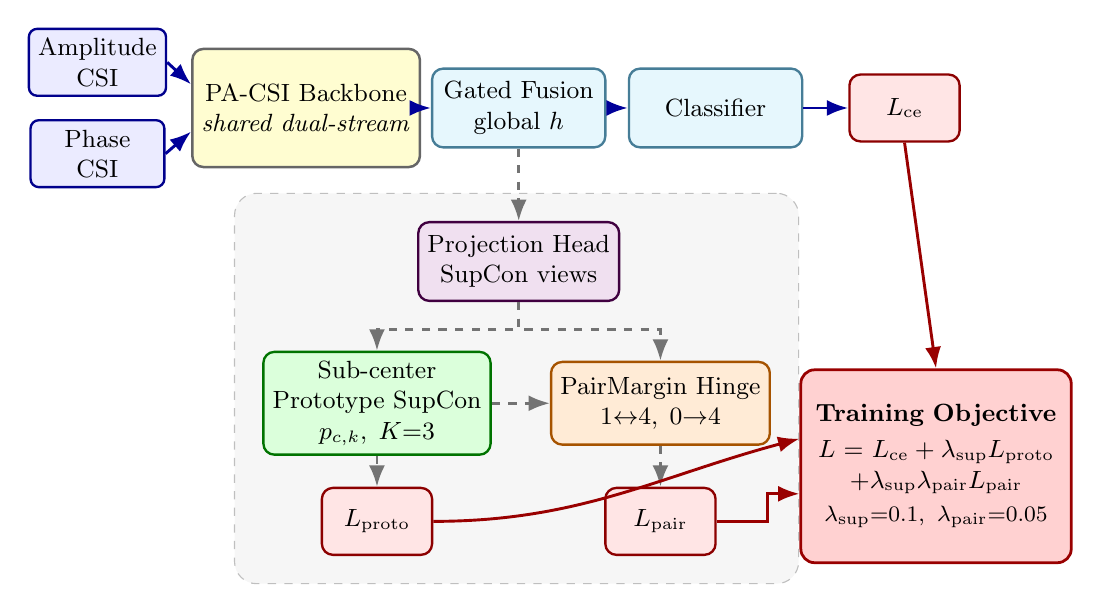
\begin{tikzpicture}[
  >=Latex, font=\small,
  io/.style    ={draw=blue!55!black, rounded corners=3pt, fill=blue!8,
                 align=center, minimum width=1.7cm, minimum height=0.85cm, line width=0.85pt},
  back/.style  ={draw=black!60, rounded corners=4pt, fill=yellow!18,
                 align=center, minimum width=2.4cm, minimum height=1.5cm, line width=0.9pt},
  feat/.style  ={draw=cyan!55!black, rounded corners=4pt, fill=cyan!10,
                 align=center, minimum width=2.2cm, minimum height=1.0cm, line width=0.85pt},
  proj/.style  ={draw=violet!50!black, rounded corners=4pt, fill=violet!12,
                 align=center, minimum width=2.5cm, minimum height=1.0cm, line width=0.85pt},
  proto/.style ={draw=green!45!black, rounded corners=4pt, fill=green!14,
                 align=center, minimum width=2.65cm, minimum height=1.3cm, line width=0.85pt},
  margin/.style={draw=orange!65!black, rounded corners=4pt, fill=orange!16,
                 align=center, minimum width=2.5cm, minimum height=1.05cm, line width=0.85pt},
  loss/.style  ={draw=red!55!black, rounded corners=4pt, fill=red!10,
                 align=center, minimum width=1.4cm, minimum height=0.85cm, line width=0.85pt},
  total/.style ={draw=red!60!black, rounded corners=5pt, fill=red!18,
                 align=center, text width=3.2cm, minimum height=2.45cm, line width=1.0pt},
  flow/.style  ={->, line width=1.05pt, draw=blue!60!black},
  tflow/.style ={->, line width=1.05pt, dashed, draw=black!55},
  lflow/.style ={->, line width=1.05pt, draw=red!60!black},
]
% Inputs and inference path -- one compact top row.
\node[io] (amp)   at (0, 0.58) {Amplitude\\CSI};
\node[io] (phase) at (0,-0.58) {Phase\\CSI};
\node[back] (backbone) at (2.65, 0) {PA-CSI Backbone\\\textit{shared dual-stream}};
\node[feat] (fus)      at (5.35, 0) {Gated Fusion\\global $h$};
\node[feat] (cls)      at (7.85, 0) {Classifier};
\node[loss] (ce)       at (10.25,0) {$L_{\mathrm{ce}}$};

% Training-only contrastive branch -- hung below fusion and split into two local paths.
\node[proj]   (proj)   at (5.35, -1.95) {Projection Head\\SupCon views};
\node[proto]  (protos) at (3.55, -3.75) {Sub-center\\Prototype SupCon\\$p_{c,k},\;K{=}3$};
\node[margin] (pair)   at (7.15, -3.75) {PairMargin Hinge\\$1{\leftrightarrow}4,\;0{\rightarrow}4$};
\node[loss]   (lp)     at (3.55, -5.25) {$L_{\mathrm{proto}}$};
\node[loss]   (lm)     at (7.15, -5.25) {$L_{\mathrm{pair}}$};

% Total objective -- lower-right, with a visible gap from the training branch box.
\node[total] (total) at (10.65,-4.55)
  {\textbf{Training Objective}\\[2pt]
   $L=L_{\mathrm{ce}}+\lambda_{\mathrm{sup}}L_{\mathrm{proto}}$\\
   $+\lambda_{\mathrm{sup}}\lambda_{\mathrm{pair}}L_{\mathrm{pair}}$\\[1pt]
   \footnotesize $\lambda_{\mathrm{sup}}{=}0.1,\;\lambda_{\mathrm{pair}}{=}0.05$};

% Inference arrows (solid blue).
\draw[flow] (amp.east)   -- ([yshift=0.3cm]backbone.west);
\draw[flow] (phase.east) -- ([yshift=-0.3cm]backbone.west);
\draw[flow] (backbone) -- (fus);
\draw[flow] (fus)      -- (cls);
\draw[flow] (cls)      -- (ce);

% Training-only arrows (dashed gray).
\draw[tflow] (fus.south) -- (proj.north);
\draw[tflow] (proj.south) -- ++(0,-0.35) -| (protos.north);
\draw[tflow] (proj.south) -- ++(0,-0.35) -| (pair.north);
\draw[tflow] (protos.south) -- (lp.north);
\draw[tflow] (protos.east) -- (pair.west);
\draw[tflow] (pair.south) -- (lm.north);

% Loss arrows into total (red).
\draw[lflow] (ce.south) -- (total.north);
\draw[lflow] (lp.east) to[out=0,in=195] ([yshift=0.35cm]total.west);
\draw[lflow] (lm.east) -- ++(0.65,0) |- ([yshift=-0.35cm]total.west);

% Soft dashed background on the training-only branch
\begin{scope}[on background layer]
  \node[draw=gray!50, dashed, rounded corners=8pt, fill=gray!7,
        inner xsep=10pt, inner ysep=10pt,
        fit=(proj)(protos)(pair)(lp)(lm)] (trainbg) {};
\end{scope}
\end{tikzpicture}%
}
\caption{PA-CSI DG model. \textbf{Top row (solid blue):} the inference path used at test time --- amplitude and phase CSI are encoded by the shared PA-CSI backbone, fused into the global feature $h$, and classified to yield $L_{\mathrm{ce}}$. \textbf{Lower region (dashed gray, highlighted box):} the training-only SupCon branch --- the projection head produces SupCon embeddings from the global representation plus three transmitter views. Instead of the old pairwise SupCon positive set, these embeddings are scored against $K{=}3$ learnable sub-centers per class to yield $L_{\mathrm{proto}}$, and a confusion-aware pair-margin hinge contributes $L_{\mathrm{pair}}$. \textbf{Red arrows:} the three loss terms summed into the training objective with weights $\lambda_{\mathrm{sup}}{=}0.1$ and $\lambda_{\mathrm{pair}}{=}0.05$.}
\label{fig:model_reminder}
\end{figure}

Mathematically, the old pairwise SupCon objective used a same-class positive set:
\[
\mathcal{L}_{\mathrm{sup}}(i)
=
-\frac{1}{|P(i)|}
\sum_{p\in P(i)}
\log
\frac{\exp(z_i^\top z_p / \tau)}
{\sum_{a\neq i}\exp(z_i^\top z_a / \tau)} .
\]
This assumes that all same-class samples and views should be pulled together. The new prototype SupCon objective instead learns $K$ centers for each class and compares each anchor to the closest center of its true class:
\[
s_{i,c}=\max_{k\le K}\cos(z_i,p_{c,k}),
\qquad
\mathcal{L}_{\mathrm{proto}}(i)
=
-\log
\frac{\exp(s_{i,y_i}/\tau)}
{\sum_c\sum_k \exp(\cos(z_i,p_{c,k})/\tau)} .
\]
For the known $E2$ confusion pairs, the pair-margin term adds:
\[
\mathcal{L}_{\mathrm{pair}}
=
\max(0,\ m + s_{i,c^-} - s_{i,y_i}),
\]
where $(y_i,c^-)$ is one of $(1,4)$, $(4,1)$, or $(0,4)$. In this run, $K=3$, $\lambda_{\mathrm{sup}}=0.1$, $\lambda_{\mathrm{pair}}=0.05$ inside the contrastive branch, and the margin values were 0.15 for $1{\leftrightarrow}4$ and 0.10 for $0{\rightarrow}4$.

\section{Why I Use $K=3$ + PairMargin for PA-CSI}

The previous section recorded \emph{what} the new objective is. This section records \emph{why} I use the successful setting from this week's run. The argument has two parts: the multi-center loss matches the multi-mode structure of PA-CSI activity classes, and the pair-margin hinge gives a local handle on confused pairs that a global loss weight cannot provide. Figure~\ref{fig:geometry} illustrates this selected geometry.

\begin{figure}[H]
\centering
\resizebox{0.95\textwidth}{!}{%
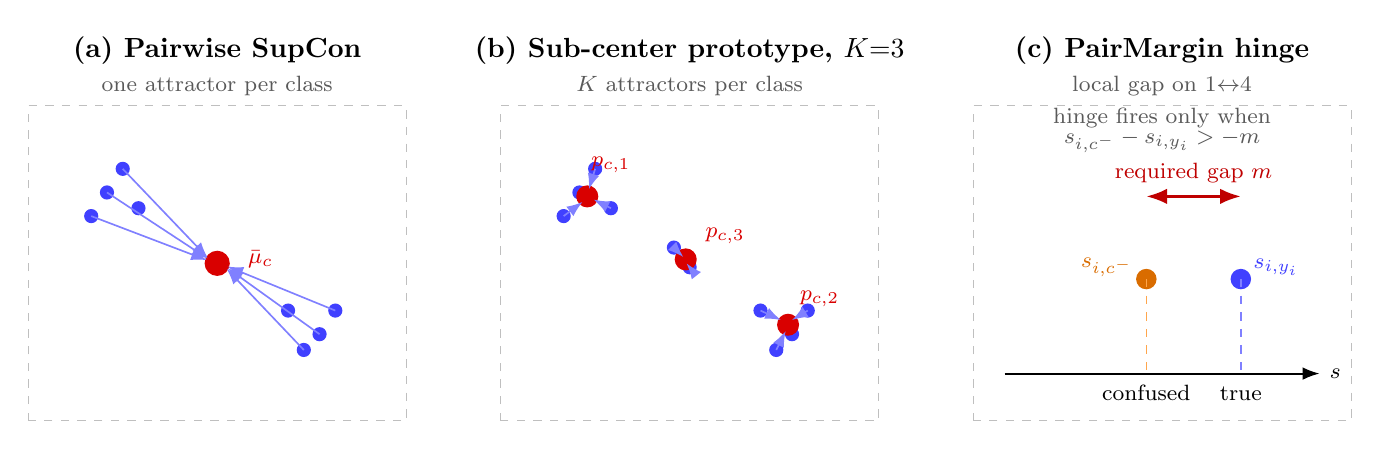
\begin{tikzpicture}[font=\small, >=Latex]
% Panel A: pairwise SupCon
\begin{scope}[shift={(0,0)}]
  \node[align=center, font=\bfseries] at (0,2.7) {(a) Pairwise SupCon};
  \node[align=center, font=\footnotesize, text=black!65] at (0,2.25) {one attractor per class};
  \draw[gray!50, dashed] (-2.4,-2.0) rectangle (2.4,2.0);
  \fill[blue!75] (-1.4, 0.9) circle (0.09);
  \fill[blue!75] (-1.2, 1.2) circle (0.09);
  \fill[blue!75] (-1.6, 0.6) circle (0.09);
  \fill[blue!75] (-1.0, 0.7) circle (0.09);
  \fill[blue!75] (1.3, -0.9) circle (0.09);
  \fill[blue!75] (1.5, -0.6) circle (0.09);
  \fill[blue!75] (1.1, -1.1) circle (0.09);
  \fill[blue!75] (0.9, -0.6) circle (0.09);
  \fill[red!85!black] (0,0) circle (0.16);
  \node[red!85!black, font=\footnotesize] at (0.55,0.05) {$\bar{\mu}_c$};
  \draw[->, blue!50, line width=0.6pt] (-1.4,0.9) -- (-0.12,0.06);
  \draw[->, blue!50, line width=0.6pt] (-1.2,1.2) -- (-0.12,0.07);
  \draw[->, blue!50, line width=0.6pt] (-1.6,0.6) -- (-0.13,0.04);
  \draw[->, blue!50, line width=0.6pt] (1.3,-0.9) -- (0.13,-0.06);
  \draw[->, blue!50, line width=0.6pt] (1.5,-0.6) -- (0.13,-0.04);
  \draw[->, blue!50, line width=0.6pt] (1.1,-1.1) -- (0.12,-0.07);
\end{scope}

% Panel B: sub-center prototype
\begin{scope}[shift={(6.0,0)}]
  \node[align=center, font=\bfseries] at (0,2.7) {(b) Sub-center prototype, $K{=}3$};
  \node[align=center, font=\footnotesize, text=black!65] at (0,2.25) {$K$ attractors per class};
  \draw[gray!50, dashed] (-2.4,-2.0) rectangle (2.4,2.0);
  \fill[blue!75] (-1.4, 0.9) circle (0.09);
  \fill[blue!75] (-1.2, 1.2) circle (0.09);
  \fill[blue!75] (-1.6, 0.6) circle (0.09);
  \fill[blue!75] (-1.0, 0.7) circle (0.09);
  \fill[blue!75] (1.3, -0.9) circle (0.09);
  \fill[blue!75] (1.5, -0.6) circle (0.09);
  \fill[blue!75] (1.1, -1.1) circle (0.09);
  \fill[blue!75] (0.9, -0.6) circle (0.09);
  \fill[blue!75] (0.0, -0.05) circle (0.09);
  \fill[blue!75] (-0.2, 0.2) circle (0.09);
  \fill[red!85!black] (-1.3,0.85) circle (0.14);
  \fill[red!85!black] (1.25,-0.78) circle (0.14);
  \fill[red!85!black] (-0.05,0.05) circle (0.14);
  \node[red!85!black, font=\footnotesize] at (-1.0,1.25) {$p_{c,1}$};
  \node[red!85!black, font=\footnotesize] at (1.65,-0.45) {$p_{c,2}$};
  \node[red!85!black, font=\footnotesize] at (0.45,0.35) {$p_{c,3}$};
  \draw[->, blue!50, line width=0.6pt] (-1.6,0.6) -- (-1.36,0.78);
  \draw[->, blue!50, line width=0.6pt] (-1.2,1.2) -- (-1.28,0.94);
  \draw[->, blue!50, line width=0.6pt] (-1.0,0.7) -- (-1.22,0.81);
  \draw[->, blue!50, line width=0.6pt] (1.5,-0.6) -- (1.30,-0.72);
  \draw[->, blue!50, line width=0.6pt] (1.1,-1.1) -- (1.22,-0.86);
  \draw[->, blue!50, line width=0.6pt] (0.9,-0.6) -- (1.16,-0.72);
  \draw[->, blue!50, line width=0.6pt] (-0.2,0.2) -- (-0.08,0.08);
  \draw[->, blue!50, line width=0.6pt] (0.0,-0.05) -- (-0.04,0.0);
\end{scope}

% Panel C: pair margin (1D similarity axis)
\begin{scope}[shift={(12.0,0)}]
  \node[align=center, font=\bfseries] at (0,2.7) {(c) PairMargin hinge};
  \node[align=center, font=\footnotesize, text=black!65] at (0,2.25) {local gap on $1{\leftrightarrow}4$};
  \draw[gray!50, dashed] (-2.4,-2.0) rectangle (2.4,2.0);
  \draw[->, line width=0.7pt] (-2.0,-1.4) -- (2.0,-1.4) node[right, font=\footnotesize] {$s$};
  \fill[blue!75] (1.0,-0.2) circle (0.13);
  \node[blue!75, font=\footnotesize] at (1.45,-0.05) {$s_{i,y_i}$};
  \draw[blue!50, dashed, line width=0.5pt] (1.0,-0.2) -- (1.0,-1.4);
  \node[font=\footnotesize] at (1.0,-1.65) {true};
  \fill[orange!85!black] (-0.2,-0.2) circle (0.13);
  \node[orange!85!black, font=\footnotesize] at (-0.7,-0.05) {$s_{i,c^-}$};
  \draw[orange!70, dashed, line width=0.5pt] (-0.2,-0.2) -- (-0.2,-1.4);
  \node[font=\footnotesize] at (-0.2,-1.65) {confused};
  \draw[<->, line width=1pt, red!75!black] (-0.2,0.85) -- (1.0,0.85);
  \node[red!75!black, font=\footnotesize] at (0.4,1.15) {required gap $m$};
  \node[font=\footnotesize, align=center, text=black!65] at (0,1.85) {hinge fires only when};
  \node[font=\footnotesize, align=center, text=black!65] at (0,1.55) {$s_{i,c^-} - s_{i,y_i} > -m$};
\end{scope}
\end{tikzpicture}%
}
\caption{Successful contrastive setting used this week, with one reference panel. \textbf{(b) and (c) are the actual configuration: $K=3$ sub-center prototypes plus PairMargin.} (b) Each class owns three learnable centers, and each anchor follows its closest one, so multimodal class structure is preserved. (c) The PairMargin hinge is a one-sided, class-conditional correction that activates only when the gap on a known confused pair shrinks below $m$, leaving well-separated classes untouched. (a) Single-attractor reference for context: pulling every same-class sample toward one centroid $\bar{\mu}_c$, the unimodal limit that motivates moving to the multi-center version in (b).}
\label{fig:geometry}
\end{figure}

\subsection*{Why I use sub-center prototypes for PA-CSI}

PA-CSI activity classes are multimodal by construction. The same activity produces different propagation paths under different body orientations and antenna combinations, and the retained transmitter views deliberately surface those modes as separate views per sample. The geometry I want is therefore one in which each class can occupy several local clusters in projection space at the same time, instead of being pulled into a single shared centroid that sits between the modes.

The sub-center prototype loss provides exactly this: it equips each class with $K$ learnable centers $p_{c,1},\dots,p_{c,K}$ and assigns each anchor to its closest center via the max-over-$k$ score
\[
s_{i,c} \;=\; \max_{k} \cos(z_i, p_{c,k}).
\]
In the low-temperature limit only the closest prototype receives the gradient, so the class manifold can stably support $K$ modes (Figure~\ref{fig:geometry}b). Cross-class repulsion is preserved by the full denominator $\sum_c\sum_k \exp(\cos(z_i,p_{c,k})/\tau)$, so prototypes belonging to different classes remain mutually pushed apart.

Two limit cases are worth keeping in mind. With $K{=}1$, the loss reduces to a standard single-prototype form, which is structurally close to pulling everything to one class centroid; this is shown in Figure~\ref{fig:geometry}(a) only as a reference for the unimodal limit. With $K \ge K^*$ (more centers than intrinsic modes), redundant prototypes either collapse onto an existing center or absorb a few outliers; the objective does not penalise unused prototypes, so over-provisioning is safe.

\subsection*{Why the pair margin is a local, asymmetric correction}

Both pairwise SupCon and the prototype log-softmax share a single denominator across all classes. They cannot independently adjust the gap between two specific classes. Increasing $\lambda_{\mathrm{sup}}$ tightens \emph{every} class boundary, including ones that were already well separated, and in our diagnostics this produced unstable trade-offs across classes. The $E2$ confusion is concentrated on $1\leftrightarrow 4$ and $0\to 4$; this is a structural property of these specific activities under $E2$, not an overall under-training signal.

The pair-margin hinge isolates these confused pairs:
\[
\mathcal{L}_{\mathrm{pair}}(i)
=
\mathrm{ReLU}\!\big(m + s_{i,c^-} - s_{i,y_i}\big)\cdot \mathbf{1}[y_i = y^\star],
\]
which is exactly zero when the gap already exceeds $m$ and otherwise applies a constant gradient until the gap is restored (Figure~\ref{fig:geometry}c). Two properties matter for our use case: it is \emph{one-sided}, so it cannot worsen well-separated classes; and it is \emph{class-conditional}, so the budget can be spent only on the pairs where the geometry actually fails.

\subsection*{Mapping to this week's experiments}

The Layer-1 design is a small-but-targeted ablation that follows directly from the analysis above:
\begin{itemize}[leftmargin=*]
  \item \textbf{$K=2$ vs.\ $K=3$, no margin.} Tests the multimodality hypothesis. If $E2$ classes are unimodal the two settings should be indistinguishable; if they are multimodal the larger $K$ should help, but only on the classes whose manifold actually has more modes.
  \item \textbf{$K=3$ no margin vs.\ $K=3$ + margin.} Tests whether the residual error after fixing geometry is structural (between specific class pairs) and therefore needs a local term, or merely a question of overall contrastive strength.
\end{itemize}

The 200-epoch confirmation run then tests whether these geometric choices remain stable under long training.

\section{Experimental Results Analysis and Comparison with Old SupCon 200e}

Table~\ref{tab:e2_200e} compares the new 200-epoch result against the previous old SupCon 200-epoch reference on target $E2$.

\begin{table}[H]
\centering
\caption{$E2$ 200-epoch comparison.}
\label{tab:e2_200e}
\small
\begin{tabular}{lccc}
\toprule
Method & Contrastive geometry & E2 Acc. & Macro-F1 \\
\midrule
Old SupCon & pairwise same-class all-view positives & 89.53 & -- \\
Sub-center prototype + PairMargin & $K=3$ prototypes + local margins & \textbf{90.23} & \textbf{88.24} \\
\bottomrule
\end{tabular}
\end{table}

\noindent The new method improves over old SupCon by 0.70 percentage points on $E2$ at the same 200-epoch budget. The key point is that the prototype method keeps the long-training benefit and becomes the strongest $E2$ result so far under the same 200-epoch comparison.

Table~\ref{tab:confusions} compares the main confusion cells. The prototype method does not uniformly improve every class. It changes the error structure in a more targeted way.

\begin{table}[H]
\centering
\caption{Key $E2$ confusion cells at 200 epochs.}
\label{tab:confusions}
\small
\begin{tabular}{lrrr}
\toprule
Method & true 1 $\rightarrow$ pred 4 & true 4 $\rightarrow$ pred 1 & true 0 $\rightarrow$ pred 4 \\
\midrule
Old SupCon & 77 & 118 & 1 \\
Sub-center prototype + PairMargin & 139 & \textbf{74} & 2 \\
\bottomrule
\end{tabular}
\end{table}

Table~\ref{tab:per_class} gives the complete per-class comparison using precision, recall, and F1. I do not report per-class accuracy because, in single-label multi-class classification, it is dominated by true negatives and is less informative than recall and F1 for class-wise behavior.

\begin{table}[H]
\centering
\caption{All-class $E2$ precision/recall/F1 comparison at 200 epochs. Higher is better.}
\label{tab:per_class}
\scriptsize
\setlength{\tabcolsep}{4pt}
\begin{tabular}{lrrrrrrr}
\toprule
Class & Old P & Old R & Old F1 & Proto P & Proto R & Proto F1 & $\Delta$F1 \\
\midrule
0 & \textbf{96.53} & 99.58 & \textbf{98.03} & 95.92 & \textbf{99.83} & 97.84 & -0.19 \\
1 & 65.58 & \textbf{75.25} & \textbf{70.08} & \textbf{73.15} & 59.25 & 65.47 & -4.61 \\
2 & \textbf{99.13} & 85.00 & 91.52 & 98.70 & \textbf{94.75} & \textbf{96.68} & +5.16 \\
3 & 97.70 & 95.75 & 96.72 & \textbf{99.50} & \textbf{98.75} & \textbf{99.12} & +2.40 \\
4 & \textbf{72.63} & 67.00 & 69.70 & 66.89 & \textbf{74.75} & \textbf{70.60} & +0.90 \\
5 & \textbf{100.00} & \textbf{99.50} & \textbf{99.75} & \textbf{100.00} & \textbf{99.50} & \textbf{99.75} & +0.00 \\
\bottomrule
\end{tabular}
\end{table}

The main gain is that class 4 becomes substantially more stable. Its recall rises from 67.00\% under old SupCon to 74.75\% under the prototype method, and the \code{4 -> 1} confusion drops from 118 to 74. Class 2 also improves strongly, with F1 rising from 91.52\% to 96.68\%, and class 3 improves from 96.72\% to 99.12\%. These gains are large enough to overcome the main negative side effect: class 1 F1 drops from 70.08\% to 65.47\%, mostly because recall falls through the larger \code{1 -> 4} confusion, even though class-1 precision increases.

The result suggests that the old SupCon geometry was too restrictive for this target. Pairwise SupCon forces all same-class views into a common cluster. The prototype loss relaxes this by allowing each activity to occupy several learned sub-centers. This is better aligned with CSI activity recognition, where the same action can have multiple stable modes under different propagation paths or antenna views. The pair-margin term then directly attacks the known local boundary instead of increasing global contrastive pressure for all classes.

The current limitation is clear: the margin helped class 4 more than class 1. The method is therefore not fully symmetric, even though the configured pair list included both $1{\rightarrow}4$ and $4{\rightarrow}1$. Future tuning should not simply increase the global loss weight; it should inspect whether class 1 needs a different margin strength, fewer prototype centers, or a class-conditional margin.

\section{Future Steps}

The next step is to move from the single-target $E2$ diagnosis to a full LOEO evaluation over all three target environments.

\begin{enumerate}[leftmargin=*]
    \item Run the selected \code{K=3 + PairMargin} configuration on full LOEO targets $E1$, $E2$, and $E3$ with seed 42, keeping the same backbone, sampler, optimizer, epoch budget, and no NARC/AdaIN.
    \item Compare the full LOEO mean accuracy and macro-F1 against the old SupCon reference: 90.27\% mean accuracy and 88.20\% mean macro-F1.
    \item Check whether the $E2$ improvement transfers or whether the pair-margin list overfits the $E2$ confusion structure. If $E1$ or $E3$ shows a new dominant confusion pair, add a separate diagnostic rather than immediately changing the full method.
    \item If the full LOEO result is positive, repeat with additional seeds. If the mean result is mixed, run a focused ablation between $K=2$ no-pair and $K=3$ PairMargin to separate the effect of sub-centers from the effect of hand-selected margins.
\end{enumerate}

\end{document}
